\documentclass[border=8pt]{standalone}
\usepackage{pgfplots}
\pgfplotsset{compat=1.18, trig format plots=deg}
\begin{document}
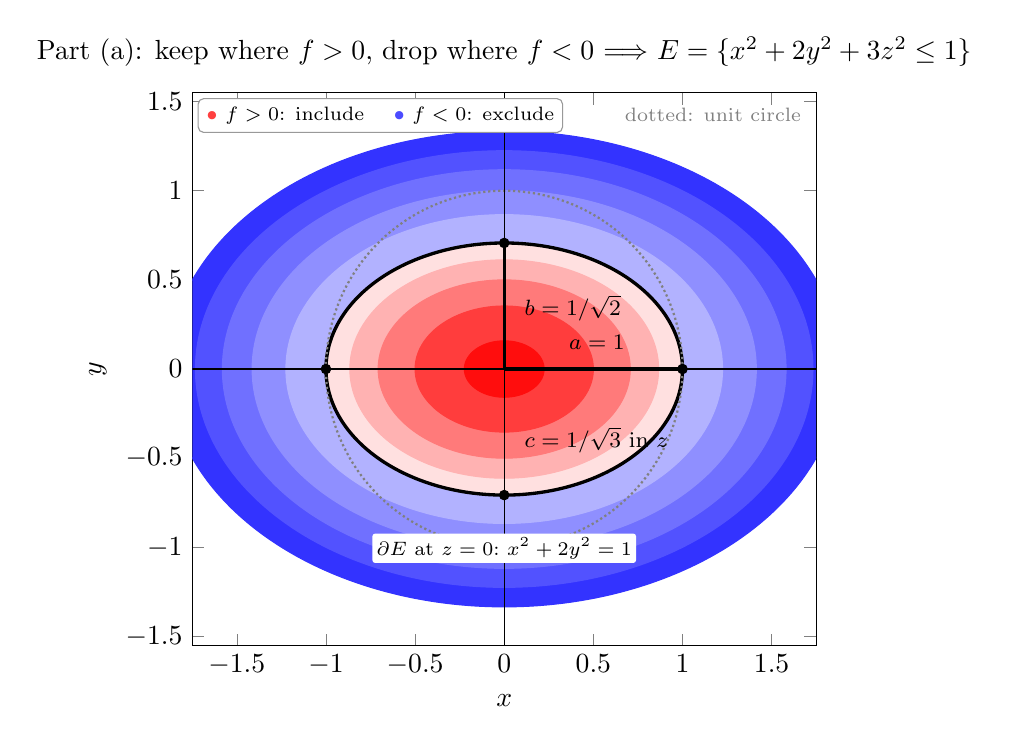
\begin{tikzpicture}
\begin{axis}[
    width  = 11.0cm, height = 8.6cm,
    axis equal image,
    xmin = -1.75, xmax = 1.75, ymin = -1.55, ymax = 1.55,
    xlabel = $x$, ylabel = $y$,
    title  = {Part (a): keep where $f>0$, drop where $f<0$
              $\Longrightarrow$ $E=\{x^2+2y^2+3z^2\le 1\}$},
    every title/.append style={font=\small},
    clip mode=individual,
]
% ---- heat map of f(x,y,0)=1-x^2-2y^2 : nested level-set ellipses ---------
\addplot[fill=blue!80, draw=blue!80, domain=0:360, samples=141, smooth]
    ({1.8868*cos(x)}, {1.3342*sin(x)});
\addplot[fill=blue!68, draw=blue!68, domain=0:360, samples=141, smooth]
    ({1.7321*cos(x)}, {1.2247*sin(x)});
\addplot[fill=blue!56, draw=blue!56, domain=0:360, samples=141, smooth]
    ({1.5811*cos(x)}, {1.1180*sin(x)});
\addplot[fill=blue!44, draw=blue!44, domain=0:360, samples=141, smooth]
    ({1.4142*cos(x)}, {1.0*sin(x)});
\addplot[fill=blue!30, draw=blue!30, domain=0:360, samples=141, smooth]
    ({1.2247*cos(x)}, {0.8660*sin(x)});
\addplot[fill=red!12, draw=red!12, domain=0:360, samples=141, smooth]
    ({1.0*cos(x)}, {0.7071*sin(x)});
\addplot[fill=red!30, draw=red!30, domain=0:360, samples=141, smooth]
    ({0.8660*cos(x)}, {0.6124*sin(x)});
\addplot[fill=red!52, draw=red!52, domain=0:360, samples=141, smooth]
    ({0.7071*cos(x)}, {0.5*sin(x)});
\addplot[fill=red!76, draw=red!76, domain=0:360, samples=141, smooth]
    ({0.5*cos(x)}, {0.3536*sin(x)});
\addplot[fill=red!95, draw=red!95, domain=0:360, samples=141, smooth]
    ({0.2236*cos(x)}, {0.1581*sin(x)});

% ---- zero level set = boundary of E (slice z=0) --------------------------
\addplot[very thick, black, domain=0:360, samples=181, smooth]
    ({cos(x)}, {sin(x)/sqrt(2)});
% ---- unit circle for scale ----------------------------------------------
\addplot[densely dotted, thick, gray, domain=0:360, samples=181, smooth]
    ({cos(x)}, {sin(x)});
% ---- coordinate axes ----------------------------------------------------
\addplot[black, thin] coordinates {(-1.75,0) (1.75,0)};
\addplot[black, thin] coordinates {(0,-1.55) (0,1.55)};
% ---- semi-axis segments + endpoints -------------------------------------
\addplot[black, very thick] coordinates {(0,0) (1,0)};
\addplot[black, very thick] coordinates {(0,0) (0,0.70710678)};
\addplot[only marks, mark=*, mark size=1.7pt, black]
    coordinates {(1,0) (-1,0) (0,0.70710678) (0,-0.70710678)};
\node[black, font=\footnotesize] at (axis cs:0.52,0.15)  {$a=1$};
\node[black, font=\footnotesize, anchor=west] at (axis cs:0.06,0.34)  {$b=1/\sqrt{2}$};
\node[black, font=\footnotesize, anchor=west] at (axis cs:0.06,-0.40) {$c=1/\sqrt{3}$ in $z$};
% ---- zone key ------------------------------------------------------------
\node[anchor=north west, font=\scriptsize, align=left, inner sep=3pt,
      draw=black!40, fill=white, rounded corners=2pt] at (axis cs:-1.72,1.52)
      {{\color{red!75}$\bullet$} $f>0$: include \quad
       {\color{blue!70}$\bullet$} $f<0$: exclude};
\node[black, font=\scriptsize, anchor=north, fill=white, inner sep=1.5pt,
      rounded corners=1pt] at (axis cs:0.0,-0.92)
      {$\partial E$ at $z=0$:\ $x^2+2y^2=1$};
\node[gray, font=\scriptsize, anchor=north east] at (axis cs:1.72,1.52)
      {dotted: unit circle};
\end{axis}
\end{tikzpicture}
\end{document}
